\documentclass[a4]{article}
\usepackage[utf8]{inputenc}
\usepackage[french]{babel}
\usepackage{listings}
\usepackage{color}
\usepackage{graphicx}
\usepackage[T1]{fontenc}
\usepackage{pdfpages}
\usepackage{geometry}
\geometry{hmargin=2.5cm,vmargin=2.5cm}

\definecolor{mygreen}{rgb}{0,0.6,0}
\definecolor{mygray}{rgb}{0.5,0.5,0.5}
\definecolor{mymauve}{rgb}{0.58,0,0.82}

\lstset{
  backgroundcolor=\color{white},   % choose the background color; you must add \usepackage{color} or \usepackage{xcolor}
  basicstyle=\footnotesize,        % the size of the fonts that are used for the code
  breakatwhitespace=false,         % sets if automatic breaks should only happen at whitespace
  breaklines=true,                 % sets automatic line breaking
  captionpos=b,                    % sets the caption-position to bottom
  commentstyle=\color{mygreen},    % comment style
  deletekeywords={...},            % if you want to delete keywords from the given language
  escapeinside={\%*}{*)},          % if you want to add LaTeX within your code
  extendedchars=true,              % lets you use non-ASCII characters; for 8-bits encodings only, does not work with UTF-8
  frame=L,	                       % adds a frame around the code
  keepspaces=true,                 % keeps spaces in text, useful for keeping indentation of code (possibly needs columns=flexible)
  keywordstyle=\color{blue},       % keyword style
  language=C,                 	   % the language of the code
  otherkeywords={*,...},           % if you want to add more keywords to the set
  numbers=none,                    % where to put the line-numbers; possible values are (none, left, right)
  numbersep=5pt,                   % how far the line-numbers are from the code
  numberstyle=\tiny\color{mygray}, % the style that is used for the line-numbers
  rulecolor=\color{black},         % if not set, the frame-color may be changed on line-breaks within not-black text (e.g. comments (green here))
  showspaces=false,                % show spaces everywhere adding particular underscores; it overrides 'showstringspaces'
  showstringspaces=false,          % underline spaces within strings only
  showtabs=false,                  % show tabs within strings adding particular underscores
  stepnumber=2,                    % the step between two line-numbers. If it's 1, each line will be numbered
  stringstyle=\color{mymauve},     % string literal style
  tabsize=2,	                   % sets default tabsize to 2 spaces
  title=\lstname                   % show the filename of files included with \lstinputlisting; also try caption= instead of title
}
%gestion des caractères latins
\lstset{literate=
  {á}{{\'a}}1 {é}{{\'e}}1 {í}{{\'i}}1 {ó}{{\'o}}1 {ú}{{\'u}}1
  {Á}{{\'A}}1 {É}{{\'E}}1 {Í}{{\'I}}1 {Ó}{{\'O}}1 {Ú}{{\'U}}1
  {à}{{\`a}}1 {è}{{\`e}}1 {ì}{{\`i}}1 {ò}{{\`o}}1 {ù}{{\`u}}1
  {À}{{\`A}}1 {È}{{\'E}}1 {Ì}{{\`I}}1 {Ò}{{\`O}}1 {Ù}{{\`U}}1
  {ä}{{\"a}}1 {ë}{{\"e}}1 {ï}{{\"i}}1 {ö}{{\"o}}1 {ü}{{\"u}}1
  {Ä}{{\"A}}1 {Ë}{{\"E}}1 {Ï}{{\"I}}1 {Ö}{{\"O}}1 {Ü}{{\"U}}1
  {â}{{\^a}}1 {ê}{{\^e}}1 {î}{{\^i}}1 {ô}{{\^o}}1 {û}{{\^u}}1
  {Â}{{\^A}}1 {Ê}{{\^E}}1 {Î}{{\^I}}1 {Ô}{{\^O}}1 {Û}{{\^U}}1
  {œ}{{\oe}}1 {Œ}{{\OE}}1 {æ}{{\ae}}1 {Æ}{{\AE}}1 {ß}{{\ss}}1
  {ű}{{\H{u}}}1 {Ű}{{\H{U}}}1 {ő}{{\H{o}}}1 {Ő}{{\H{O}}}1
  {ç}{{\c c}}1 {Ç}{{\c C}}1 {ø}{{\o}}1 {å}{{\r a}}1 {Å}{{\r A}}1
  {€}{{\EUR}}1 {£}{{\pounds}}1
}
%definition d'un syle pour les documents text
\lstdefinestyle{txt}{
	frame=none,
	numbers=none,
	stringstyle=\color{black},
}

\begin{document}
	\title{\Huge{\textbf{Manuel d'utilisation}}}
	\author{Dcrypt}
	\date{29 mai 2017}
		

	\begin{titlepage}
		\maketitle
		\vspace{20em}
		%\begin{center}\includegraphics{logo_uvsq.jpg}\end{center}
	\end{titlepage}
	\section{Introduction}
L'application Dcrypt est un outil automatique d'aide au decryptage permettant a son utilisateur d'effectuer une cryptanalyse
sur un fichier ou texte à partir d'un ordinateur. Pour cela, le procédé de Vigenère ou de Substitution lui sera proposé. \\
Le client pourra aussi effectuer le cryptage à l'aide de ces 2 methodes ou encore lancer seulement une analyse frequentielle. \\
L’application se veut très simple d’utilisation. Ce guide a été concu afin de repondre à toutes les questions d'utilisation que
pourrait avoir le client.


	\section{Pré-conditions/Materiel necessaire}

		\subsection{Installations requises}
			Certaines installations sont essentielles a l'utilisation de l'application.\\
			Tout d'abord, celle de la bibliotheque GTK: sudo apt-get install libgtk2.0-dev \\
			Enfin, pour Cunit:  sudo apt-get install libcunit1 libcunit1-doc libcunit1-dev \\

		\subsection{Lancement de l'application}
			commande pour lancer appli: make run \\
			commande pour lancer tests:make test\\


	\section{Guide d'utilisation}
	
	
	Ce guide pratique a pour objectif de vous guider dans l’utilisation de l’application
"Dcrypt" et de répondre aux éventuelles questions que vous pourriez vous poser au
cours de son usage. 
	
	

	\section{Menu/Acceuil}
			Ici, vous vous trouvez sur le menu ou page d'acceuil de l'application. \\
			Vous pouvez a l'aide de nos 3 boutons Crypter Decrypter ou faire une analyse sur un texte  \\
			\begin{center}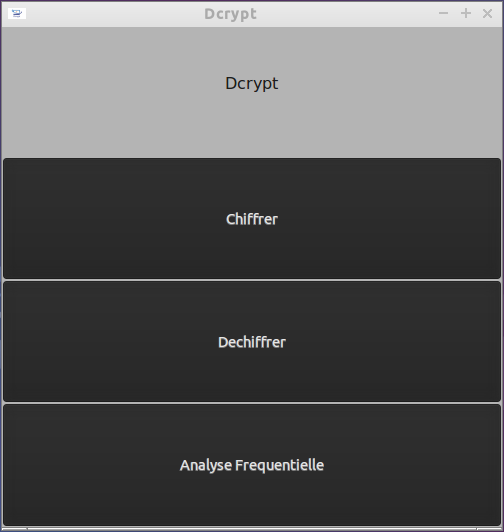
\includegraphics[scale=0.4]{1.png}\end{center}
			
			
			
	\section{Menu Cryptage}
		dans le menu cryptage vous pouvez soit choisir le type de cryptage (methode) ou 
		sinon vous avez le bouton R qui permet de revenir au menu precedent
		\begin{center}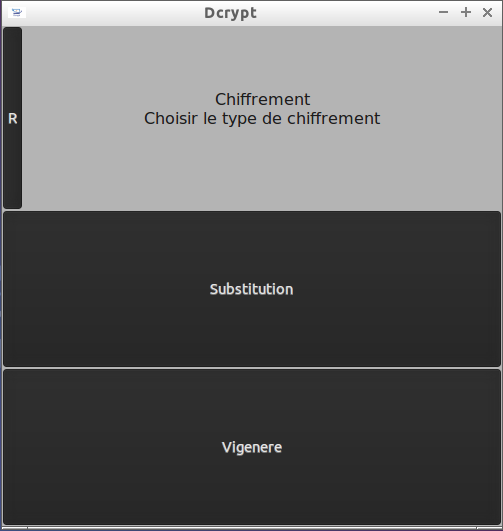
\includegraphics[scale=0.4]{2.png}\end{center}
		\subsection{Cryptage Substitution}
			la vous pouvez soit rentrer votre texte a l'aide de la zone d'entrée(8)
			soit le charger a l'aide de la fenetre de chargement (9)
			\begin{center}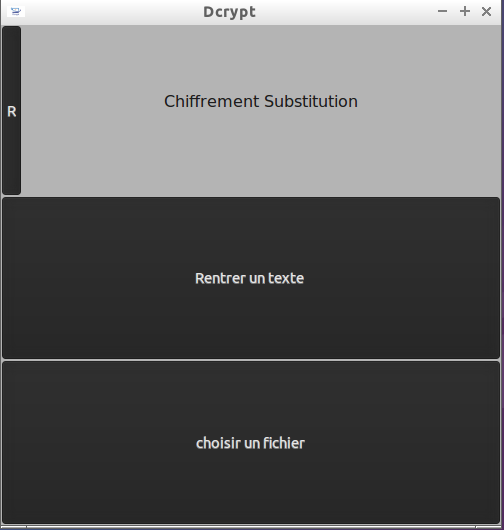
\includegraphics[scale=0.4]{3.png}\end{center}
			le resultat sera affiché \\
			vous pouvez maintenant enregistrer la clée et le texte chiffré a laide 
			de la fenetre d'enregistrement(9)
			\begin{center}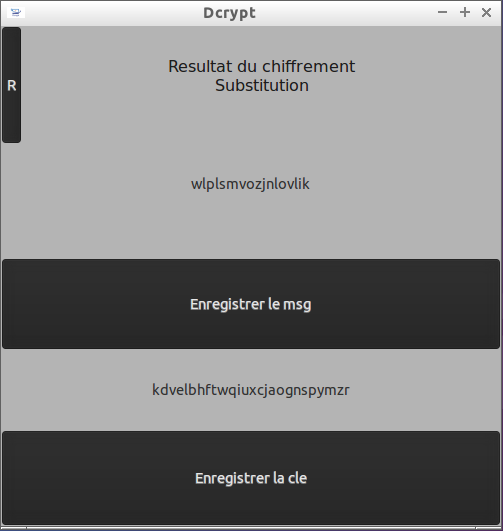
\includegraphics[scale=0.4]{5.png}\end{center}
		\subsection{Cryptage Vigenere}
		dans ce menu on vous demande tout dabord d'entrer la clé de cryptage (elle 
		doit contenir que des lettres)
			\begin{center}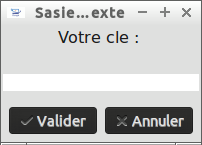
\includegraphics[scale=0.4]{22.png}\end{center}
			la vous pouvez soit rentrer votre texte a l'aide de la zone d'entrée(8)
			soit le charger a l'aide de la fenetre de chargement (9)
			\begin{center}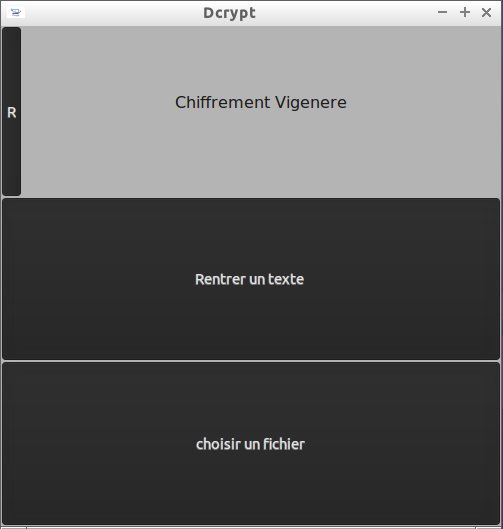
\includegraphics[scale=0.4]{6.png}\end{center}
			le resultat sera affiché \\
			vous pouvez maintenant enregistrer la clée et le texte chiffré a laide 
			de la fenetre d'enregistrement(9)
			\begin{center}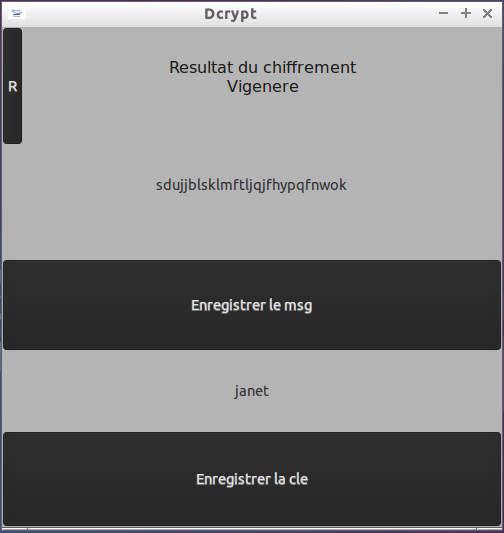
\includegraphics[scale=0.4]{7.png}\end{center}
		
		
	\section{Menu Decryptage}
		avant de commencer le decryptage vous devez donner la langue du text que vous voulez decrypter car 
		les resources en francais et en anglais ne sont pas les memes
		\begin{center}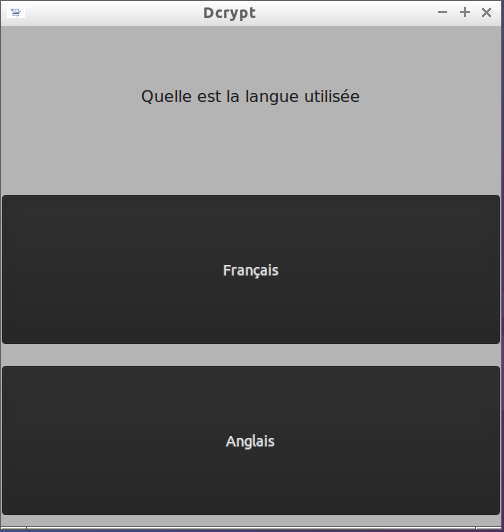
\includegraphics[scale=0.4]{8.png}\end{center}
		dans le menu decryptage vous pouvez soit choisir le type de decryptage (methode) ou 
		sinon vous avez le bouton R qui permet de revenir au menu principal
		\begin{center}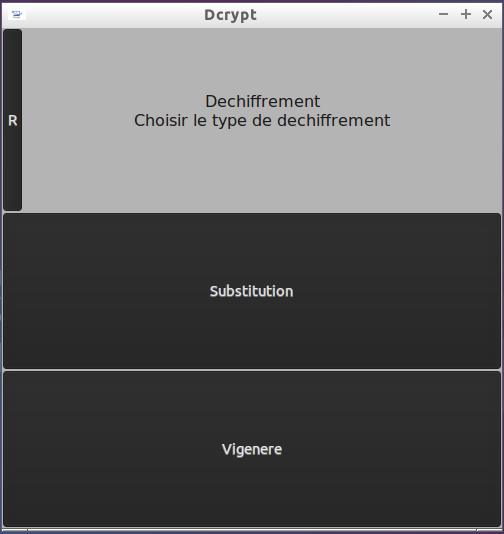
\includegraphics[scale=0.4]{9.png}\end{center}
		\subsection{Decryptage Substitution}
			la vous pouvez soit rentrer votre texte a l'aide de la zone d'entrée(8)
			soit le charger a l'aide de la fenetre de chargement (9)
			\begin{center}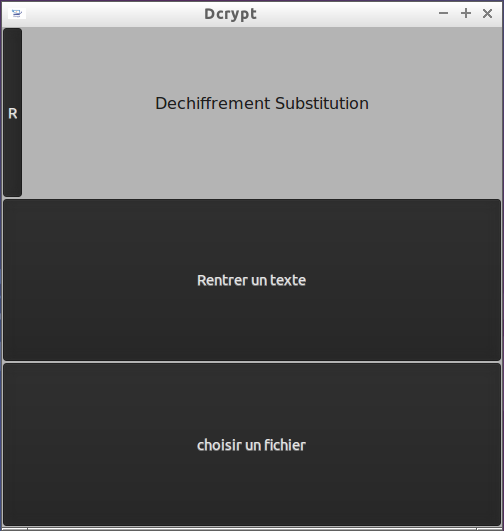
\includegraphics[scale=0.4]{10.png}\end{center}
			maintenant vous avez une partie de la clée qui est decrypter et vous allez 
			essayer de trouver quelques autres caracteres ,exemple si le resultat est :
			kONvOUR... vous pouvez etre sur que k correspond a B et v a J 
			\begin{center}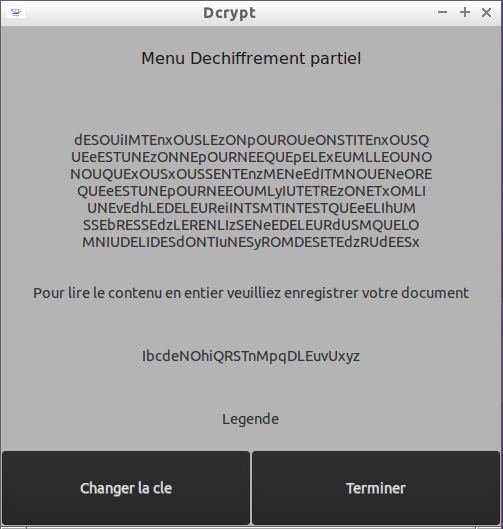
\includegraphics[scale=0.4]{13.png}\end{center}
			vou pouvez faire les modifications avec le menu changer clée 
			il manque un screen ICI
			au bout de 4 ou 5 caractéres retrouvés le texte sera decryptée (car plus de la moitier 
			des caracteres est decryptée par l'application) et vous aurez:
			\begin{center}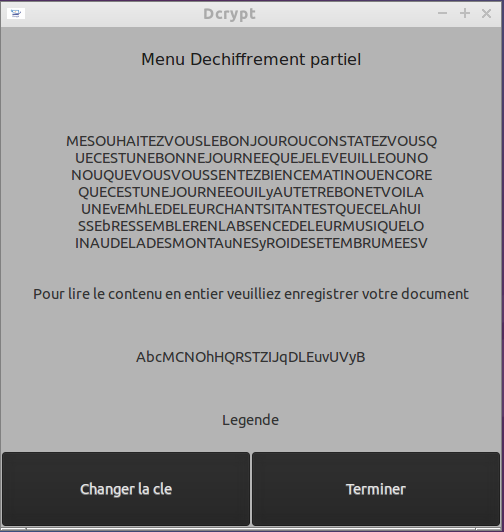
\includegraphics[scale=0.4]{11.png}\end{center}
			vous pouvez cliquer sur terminer qui vous emmenera sur ce menu qui vous permet comme pour 
			les cryptages d'enregistrer le resultat et la clée
			\begin{center}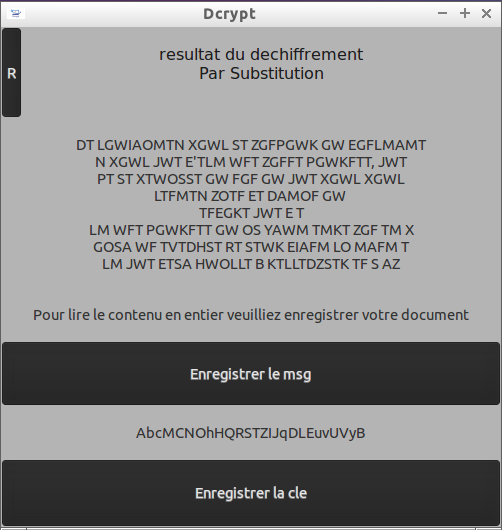
\includegraphics[scale=0.4]{12.png}\end{center}
		\subsection{Decryptage Vigenere}
			la vous pouvez soit rentrer votre texte a l'aide de la zone d'entrée(8)
			soit le charger a l'aide de la fenetre de chargement (9)
			\begin{center}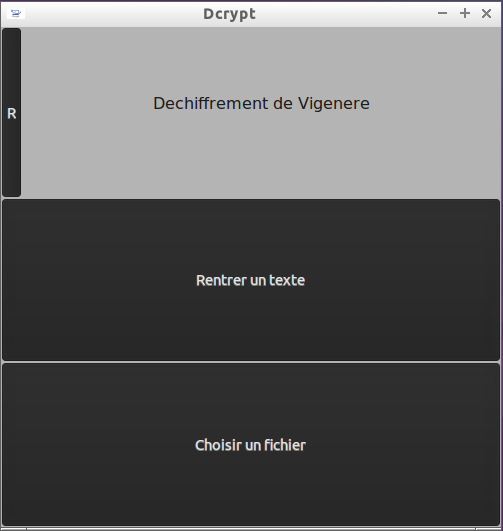
\includegraphics[scale=0.4]{14.png}\end{center}
			la vous avez une cle et un texte decrypté normalement la clé obtenu est la bonne
			si le texte et assez long si le texte est illisible alors la clé est incorrecte et
			 dans ce cas il suffit de choisir le bouton redechiffrer qui va ressayer avec une 
			 autre taille de clé . une fois le resultat trouvé vous pouvez a l'aide du bouton 
			 terminer aller au menu de resultat final.  
			\begin{center}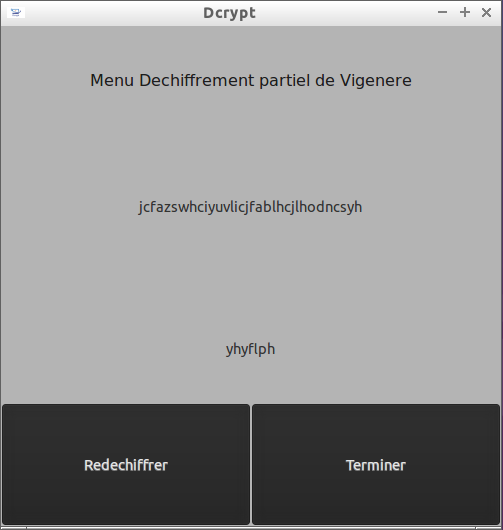
\includegraphics[scale=0.4]{15.png}\end{center}
			ce menu vous permet comme pour 
			les cryptages d'enregistrer le resultat et la clée
			\begin{center}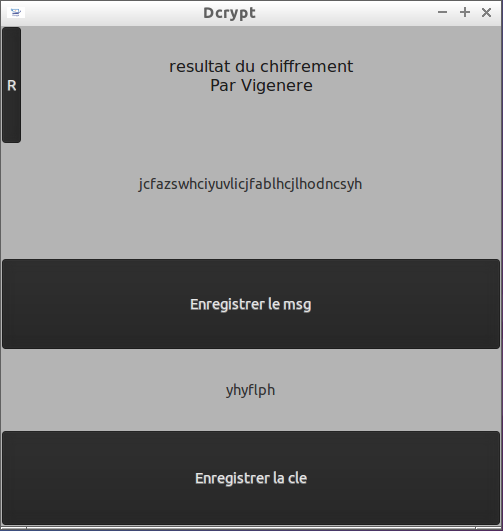
\includegraphics[scale=0.4]{16.png}\end{center}
		
		
	\section{Menu Analyse Frequentielle}
			la vous pouvez soit rentrer votre texte a l'aide de la zone d'entrée(8)
			soit le charger a l'aide de la fenetre de chargement (9)
		\begin{center}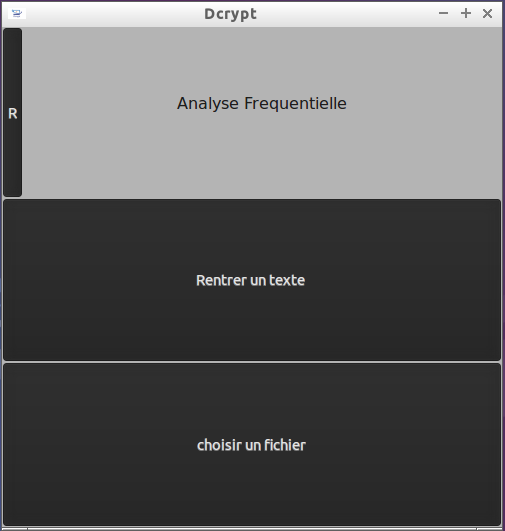
\includegraphics[scale=0.4]{17.png}\end{center}
			ensuite vous aurez les frequences de chaque lettre de l'alphabet ainsi que
			celle de chaque digramme et trigramme de lettres dans votre texte
			(si le texte est tres long elle n'affichera que ceux qui se repettent le plus)
		\begin{center}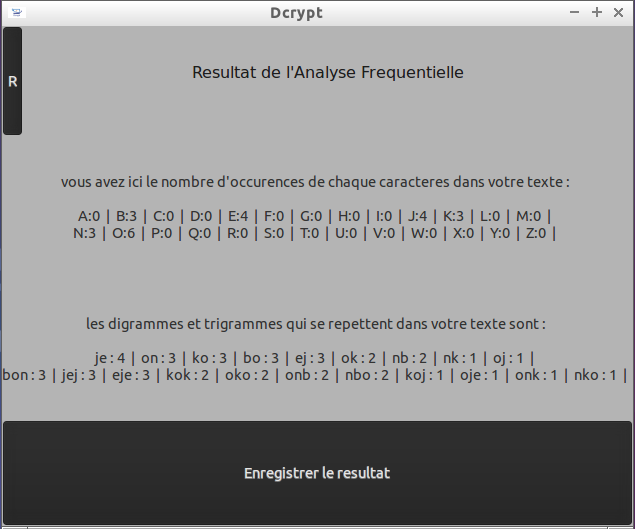
\includegraphics[scale=0.4]{18.png}\end{center}
	\section{Entrer un texte}
		a chaque fois que vous allez essayer de rentrer un texte cette fenetre va s'afficher devant vous
		\begin{center}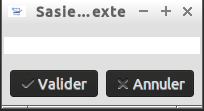
\includegraphics[scale=0.4]{21.png}\end{center}
	\section{les Chargements/Enregistrement de fichiers}
		a chaque fois que vous allez essayer de charger un texte cette fenetre aparaitre.
		\begin{center}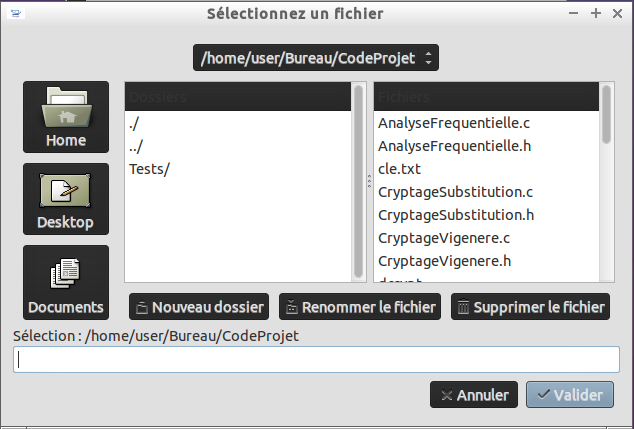
\includegraphics[scale=0.4]{19.png}\end{center}
		a chaque fois que vous allez essayer d'enregistrer un texte cette fenetre va s'afficher devant vous.
		\begin{center}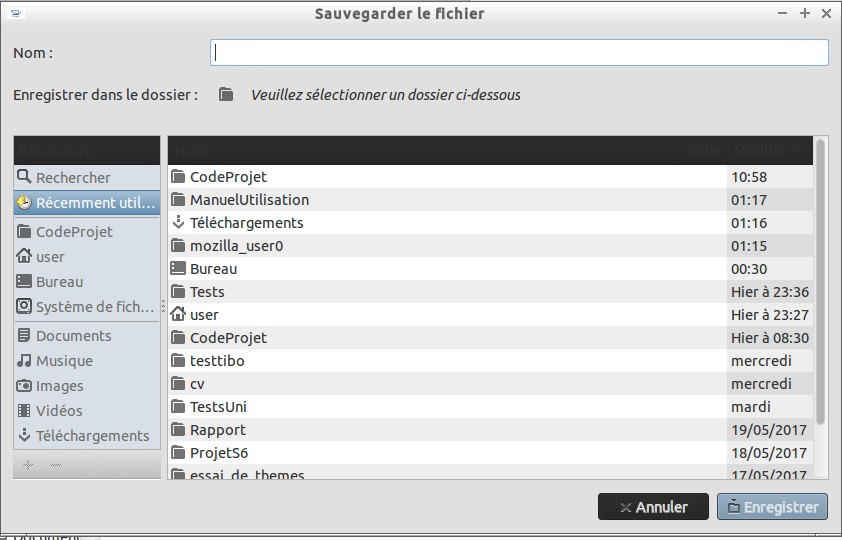
\includegraphics[scale=0.4]{20.png}\end{center}
\end{document}
